\documentclass{article}

% if you need to pass options to natbib, use, e.g.:
%     \PassOptionsToPackage{numbers, compress}{natbib}
% before loading neurips_2026

% The authors should use one of these tracks.
% Before accepting by the NeurIPS conference, select one of the options below.
% 0. "default" for submission
 \usepackage{neurips_2026}
% the "default" option is equal to the "main" option, which is used for the Main Track with double-blind reviewing.
% 1. "main" option is used for the Main Track
%  \usepackage[main]{neurips_2026}
% 2. "position" option is used for the Position Paper Track
%  \usepackage[position]{neurips_2026}
% 3. "dandb" option is used for the Datasets & Benchmarks Track
 % \usepackage[dandb]{neurips_2026}
% 4. "creativeai" option is used for the Creative AI Track
%  \usepackage[creativeai]{neurips_2026}
% 5. "sglblindworkshop" option is used for the Workshop with single-blind reviewing
 % \usepackage[sglblindworkshop]{neurips_2026}
% 6. "dblblindworkshop" option is used for the Workshop with double-blind reviewing
%  \usepackage[dblblindworkshop]{neurips_2026}

% After being accepted, the authors should add "final" behind the track to compile a camera-ready version.
% 1. Main Track
 % \usepackage[main, final]{neurips_2026}
% 2. Position Paper Track
%  \usepackage[position, final]{neurips_2026}
% 3. Datasets & Benchmarks Track
 % \usepackage[dandb, final]{neurips_2026}
% 4. Creative AI Track
%  \usepackage[creativeai, final]{neurips_2026}
% 5. Workshop with single-blind reviewing
%  \usepackage[sglblindworkshop, final]{neurips_2026}
% 6. Workshop with double-blind reviewing
%  \usepackage[dblblindworkshop, final]{neurips_2026}
% Note. For the workshop paper template, both \title{} and \workshoptitle{} are required, with the former indicating the paper title shown in the title and the latter indicating the workshop title displayed in the footnote.
% For workshops (5., 6.), the authors should add the name of the workshop, "\workshoptitle" command is used to set the workshop title.
% \workshoptitle{WORKSHOP TITLE}

% "preprint" option is used for arXiv or other preprint submissions
 % \usepackage[preprint]{neurips_2026}

% to avoid loading the natbib package, add option nonatbib:
%    \usepackage[nonatbib]{neurips_2026}

\usepackage[utf8]{inputenc} % allow utf-8 input
\usepackage[T1]{fontenc}    % use 8-bit T1 fonts
\usepackage{hyperref}       % hyperlinks
\usepackage{url}            % simple URL typesetting
\usepackage{booktabs}       % professional-quality tables
\usepackage{amsmath}        % math support
\usepackage{amsfonts}       % blackboard math symbols
\usepackage{nicefrac}       % compact symbols for 1/2, etc.
\usepackage{microtype}      % microtypography
\usepackage{xcolor}         % colors
\usepackage{graphicx}

% Note. For the workshop paper template, both \title{} and \workshoptitle{} are required, with the former indicating the paper title shown in the title and the latter indicating the workshop title displayed in the footnote. 
\title{Sample-Efficiency of DeepRL Using Kolmogorov–Arnold Networks}

% The \author macro works with any number of authors. There are two commands
% used to separate the names and addresses of multiple authors: \And and \AND.
%
% Using \And between authors leaves it to LaTeX to determine where to break the
% lines. Using \AND forces a line break at that point. So, if LaTeX puts 3 of 4
% authors names on the first line, and the last on the second line, try using
% \AND instead of \And before the third author name.

\author{%
  % David S.~Hippocampus\thanks{Use footnote for providing further information
  %   about author (webpage, alternative address)---\emph{not} for acknowledging
  %   funding agencies.} \\
  % Department of Computer Science\\
  % Cranberry-Lemon University\\
  % Pittsburgh, PA 15213 \\
  % \texttt{hippo@cs.cranberry-lemon.edu} \\
  % examples of more authors
  % \And
  Kevin Riehl \\
  ETH Zürich, IVT \& \\
  Agentic Systems Lab (ASL) \\
  \texttt{kriehl@ethz.ch} \\
  \And
  Shaimaa K. El-Baklish \\
  ETH Zürich, IVT \\
  \texttt{selbaklish@ethz.ch} \\
  \And
  Anastasios Kouvelas \\
  ETH Zürich, IVT \\
  \texttt{kouvelas@ethz.ch} \\
}

\begin{document}

\maketitle


%%%%%%%%%%%%%%%%%%%%%%%%%%%%%%%%%%%%%%%%%%%%%%%%%%%%%%%%%%%%
\begin{abstract}
Deep reinforcement learning has achieved substantial performance gains over classical control approaches.
Yet, a central challenge to learning in real-world applications is acquiring costly samples.
Kolmogorov-Arnold Networks are a recently proposed architecture, that can particularly well learn physical relationships for control problems, with significantly higher parameter efficiency and interpretability when compared to Multi-Layer-Perceptron architectures.
In this work, we systematically study sample-efficiency using computational experiments, covering the Feynman dataset and the Gymnasium RL benchmark.
The results show, that similar performance can be achieved with 40\% less samples using the Kolmogorov-Arnold architecture, and that relative performance improvements up to 50\% during the training process.
The observed gains are robust to varying levels of noise in rewards.
These results highlight the potential of the Kolmogorov-Arnold architectures for more sample-efficient reinforcement learning.
\end{abstract}



%%%%%%%%%%%%%%%%%%%%%%%%%%%%%%%%%%%%%%%%%%%%%%%%%%%%%%%%%%%%
\section{Introduction}

%%% PARAGRAPH 01: RL-based control (using Neural Networks) is great and outperforms
Reinforcement learning (RL) has become a powerful paradigm for learning feedback controllers directly from system interactions~\cite{sutton2018reinforcement}.
Classical control methods, including model-based and model predictive control, can be highly effective when accurate models dynamics and tractable objectives are available, but these assumptions are often difficult to satisfy in complex, nonlinear, and noisy environments~\cite{kiumarsi2017optimal}.
Value-based RL methods such as Q-learning instead learn an action-value function that estimates the long-term return of taking an action in a given state~\cite{watkins1992qlearning}.
Deep RL extends this idea by replacing tabular value functions or policies with neural networks, enabling controllers to approximate high-dimensional and nonlinear state-action relationships~\cite{mnih2015humanlevel,schulman2017ppo}.
This flexibility has made neural RL attractive for control tasks in robotics, networking, and other cyber-physical systems where the controller must cope with sensor noise, nonlinear dynamics, delayed effects, and changing operating conditions.

%%% PARAGRAPH 02: What are challenges to RL-based control?
A central challenge for RL in control is the need to balance exploration and exploitation while learning from limited interactions~\cite{Zhangetal2021}.
Additional challenges include designing reward functions that encode the intended behavior and maintaining stability while the data distribution changes with the policy~\cite{eschmann2021reward}.
For safety-critical control, an additional limitation is that standard neural policies are difficult to inspect, verify, or translate into controller equations~\cite{Lietal2025}.
These issues motivate function approximators that can learn strong policies from fewer interactions while retaining enough structure to support analysis and interpretation~\cite{ferrari2005smooth}.
The most central practical challenge is that learning a useful controller can require a large number of environment interactions~\cite{zhang2021sample}.
Each sample in a control problem is not merely a labeled example, but a transition generated by running a policy in a simulator, a digital twin, or a physical system~\cite{tao2022digital}.
When running an RL environment is computationally expensive, slow, unsafe, or subject to hardware wear, sample inefficiency becomes a practical barrier to deployment.

%%% PARAGARAPH 03: TALK ABOUT KOLOMOGOROV ANROLD NETWORKS
Kolmogorov-Arnold Networks (KANs) are a recently proposed class of neural network architectures inspired by the Kolmogorov-Arnold representation theorem, which states that any continuous multivariate function can be expressed as a finite superposition of univariate functions and summation operators \cite{kolmogorov1956representation, arnold1963representation}.
Unlike traditional neural networks such as multilayer perceptrons (MLPs), which rely on linear transformations followed by fixed nonlinear activation functions, KANs replace scalar weights with learnable univariate functions defined along the edges of the network and require exactly two hidden layers~\cite{liu2024kan}.
This formulation allows the model to directly learn functional relationships between variables rather than approximating them only through weighted sums of fixed activation functions.
As a result, KANs offer improved interpretability and significantly higher parameter efficiency while retaining strong approximation capabilities.
Recently, KANs have gained considerable attention, particularly in areas where understanding the underlying functional structure of the data is important \cite{somvanshi2025survey,essahraui2025kanoverview,sohail2024training}.
KANs are therefore particularly well suited for applications such as symbolic regression, scientific discovery, and physics-informed modeling, where both data efficiency and model transparency are essential \cite{somvanshi2025survey,essahraui2025kanoverview}.
These properties have also motivated the use of KANs in RL-based control, including PPO-based continuous control, robotic policy learning, load balancing, and explainable RL \cite{kich2024online,bayeh2026kanppo,chen2025kanpolicy,singh2026loadbalancing,dalto2025explainable}.

%%% PARAGRAPH 04: TALK ABOUT RESEARCH OF KANS REGARDING SAMPLE-EFFICIENCY
Existing evidence on the efficiency of KANs is promising.
Prior work reports that smaller KANs can match or outperform larger MLPs in several data-fitting and scientific-computing examples, suggesting favorable neural scaling behavior and parameter efficiency \cite{liu2024kan}.
In structured settings, KANs have been shown to reduce the need for expensive high-fidelity data and to perform well in low-data industrial fault detection \cite{howard2024multifidelity,villagomez2025kanae,wang2025quadkan}.
Theoretical work also gives sample-complexity guarantees for residual KANs under smoothness and noiseless-sample assumptions \cite{kratsios2025besov}.
Yet, in more systematic low-data comparisons, MLPs with individualized learnable activations can outperform KANs when only a few hundred samples are available \cite{pourkamali2025lowdata}.
These mixed findings, together with the absence of a systematic assessment of sample efficiency in RL-based control applications, motivate this work: it remains unclear when KANs improve sample efficiency over MLPs under comparable experimental budgets.

%%% PARAGRAPH 05: MOTIVATION FOR RESEARCH QUESTION
Using the Feynman dataset (a collection of physical equations) and the Gymnasium RL bench (a collection of RL environments)~\citep{towers2026gymnasium} we systematically assess sample efficiency of KANs as function approximators when compared to MLPs. 
Our results show that 40\% less samples are required to achieve similar performance, and that 50\% reward gains can be achieved during the training process using KANs.  





%%%%%%%%%%%%%%%%%%%%%%%%%%%%%%%%%%%%%%%%%%%%%%%%%%%%%%%%%%%%
\section{Related Works}

\textbf{Kolmogorov--Arnold networks and learning guarantees.}
KANs were introduced as an alternative to MLPs in which learnable univariate functions are placed on edges rather than fixed nonlinearities on nodes \cite{liu2024kan}.
This architecture has motivated rapid follow-up work because it connects neural approximation to interpretable function decompositions and can use fewer parameters in some scientific-computing and symbolic-regression settings \cite{somvanshi2025survey,essahraui2025kanoverview}.
Theoretical work has begun to formalize these intuitions by proving approximation and sample-complexity guarantees for residual KANs on smooth function classes (including Besov spaces) \cite{kratsios2025besov}.
These guarantees are important, but they are typically stated under assumptions that differ from RL control, where targets are noisy, bootstrapped, and induced by a changing policy.

\textbf{Low-data and fixed-sample empirical comparisons.}
Empirical evidence for KAN sample efficiency remains mixed.
The original KAN experiments show favorable scaling and strong performance with compact models, but they do not isolate environment-sample efficiency under fixed compute and fixed interaction budgets \cite{liu2024kan}.
Follow-up works directly study low-data regimes and find that MLPs with individualized learnable activations can outperform KANs with substantially fewer parameters, especially when only a few hundred samples are available \cite{pourkamali2025lowdata}.
Further studies show that KANs and MLPs trade advantages across regular, irregular, discontinuous, and noisy functions, with KANs converging quickly in some cases but failing to dominate across stabilized test loss \cite{zeng2024irregular}.
These comparisons suggest KANs should not be treated as universally more sample-efficient than MLPs.

\textbf{Structured and expensive-data settings.}
More positive results appear when the problem structure matches the inductive bias of KAN edge functions.
Some works propose multifidelity KANs that combine abundant low-fidelity data with limited high-fidelity data, reducing the amount of expensive high-fidelity data needed in scientific machine learning \cite{howard2024multifidelity}.
Furthermore, studies evaluate KAN autoencoders for fault detection across varying training-set sizes and find that several KAN variants match or surpass an MLP-based orthogonal autoencoder with substantially less data \cite{villagomez2025kanae}.
These results are highly relevant for control domains with costly simulation or measurement, but they are supervised or unsupervised learning studies rather than online RL studies.

\textbf{KANs in RL and control.}
Several recent works integrate KANs into RL pipelines.
Prior works replace MLP actor and critic components in PPO with KANs and report comparable performance with fewer parameters on DeepMind Control Proprio robotics benchmarks \cite{kich2024online}.
Similarly, studies propose KAN-PPO and MultKAN-PPO for continuous control, finding robust performance across several configurations while noting sensitivity to dropout design \cite{bayeh2026kanppo}.
Other studies focus on KAN-based PPO agents for CartPole and radio-access-network control, showing that KAN agents can match MLP performance with far fewer parameters and can be converted into sparse symbolic policies \cite{dalto2025explainable}.
Moreover, works propose a KAN actor in PPO for load balancing and emphasize the ability to extract interpretable controller equations \cite{singh2026loadbalancing}.
Together, these works support the feasibility of KAN-based RL, but they primarily emphasize parameter efficiency and interpretability rather than controlled sample-efficiency comparisons.

\textbf{KANs for robotic policies and world models.}
KANs have also been used in policy-learning systems outside the standard actor-critic replacement setting.
KAN Policy can be used for diffusion-based visuomotor policy learning, and works doing so report smoother trajectories, shorter execution times, and improved success rates relative to diffusion-policy baselines \cite{chen2025kanpolicy}.
\textit{QuadKAN} for vision-guided quadruped locomotion reports faster convergence, improved returns, lower action jitter, and better robustness in structured gait-control settings \cite{wang2025quadkan}.
\textit{KAN-Dreamer} \cite{shi2025kandreamer} replaces selected components with KAN or FastKAN \cite{li2024kolmogorovarnold} modules, finding that FastKAN is promising for reward and continue prediction but that direct replacement of visual encoders or actor-critic modules can harm sample efficiency.
This component-level evidence reinforces the need to distinguish where KANs are useful in a RL stack rather than assuming that every MLP can be replaced beneficially.




%%%%%%%%%%%%%%%%%%%%%%%%%%%%%%%%%%%%%%%%%%%%%%%%%%%%%%%%%%%%
\section{Experiments}

\subsection{Feynman Sample-Efficiency Benchmark}
The first experiment tests the core approximation question in a controlled supervised setting, before moving to full RL control.
If KANs are more sample-efficient because their edge functions provide a useful inductive bias, this advantage should already be visible when learning smooth physical laws from few samples.
For this purpose, we follow Liu et al. and use the Feynman benchmark, which contains closed-form physics equations derived from the Feynman Lectures and related symbolic-regression benchmarks \cite{liu2024kan,udrescu2020aifeynman,udrescu2020aifeynman2}.
Each benchmark task is a regression problem, where each Feynman Lecture equation is independently sampled to generate training sets (varying size) and test sets (fixed size).
The primary evaluation metric is root mean squared error (RMSE).

\subsection{RL Gymnasium Benchmark}
The second experiment studies the sample efficiency of KANs and MLPs in the context of DeepRL for control.
For this purpose, we use the RL benchmark "\textit{Gymnasium}"~\citep{towers2026gymnasium}, which contains a multitude of different physics environment to study RL.
We chose the subset of "Classic Control" as state variables are used for learning, rather than image or video streams, as KANs are known to be particularly suitable to learn physical relationships.
Furthermore, we chose the proximal policy optimization (PPO) learning strategy, as it is a standard, robust policy-gradient method for continous and discrete control problems~\citep{schulman2017proximal}.
Following environments are included in the benchmark:
"Acrobot-v1", "CartPole-v1", "MountainCar-v0", "MountainCarContinuous-v0", and "Pendulum-v1".
Each benchmark task provides a comparable learning curve with best rewards achievable (convergence limits) enabling a comparison.

\subsection{RL Gymnasium Benchmark With Noised Rewards}
The third experiment studies the robustness of the sample efficiency gains of KANs over MLPs in the context of DeepRL in control applications, for varying reward noise levels (Gaussian noise with increasing magnitudes).

\subsection{Comparison and Sample-Efficiency Assessment}
Different model complexities and training parameters were explored via grid-search to identify optimal performance.
KAN and MLP models where matched by model complexity measured in number of parameters to ensure a fair comparison.
Number of training samples (e.g., Feynman samples, or environment episodes) to achieve a certain performance were used to assess the enhanced sample-efficiency of KANs over MLPs.
Specifically, we compare ReLU and Sigmoid for MLP, and B-Splines and radial base functions (RBF) for KAN networks, to cover a multitude of different function space shapes.


%%%%%%%%%%%%%%%%%%%%%%%%%%%%%%%%%%%%%%%%%%%%%%%%%%%%%%%%%%%%
\section{Results}

% - The experiment on the Feynman benchmark (Fig.~\ref{fig:experiment_1_results}) shows gains from 5 samples onwards. Then, the NRMSE improvement increases up to 40\%.
% - Moreover, KANs fit the benchmark better than MLPs do.
% - Also, similar NRMSE performance can be achieved using KANs with 60\% less samples when compared to MLPs.
%
% - The RL experiment using the Gynmasium benchmark (Fig.~\ref{fig:experiment_2_results}) shows similar results. The different environments have different improvements and sample reducitons, but average shows similar reuslts like previous experiment.
% - Up to 50\% control performance improvement can be achieved with KANs (when compared to MLPs) during the training process.
% - the performance improvement grows after few samples and then after its peak of 3000 episodes, shrinks again.
% - In terms of sample reduction, across experiments, up to 40\% less samples are needed to achieve same performance of MLPs with KANs (at same model complexity).
% - no major performance differences are observable after great number of samples, then both MLPs and KANs perform similarly well.
%
% - The third experiment with noise around reward function demonstrates the robustness of the performance gains of KANs. Across the different noise levels, no significant differences can be observed, just variance of the experiment increased.
The Feynman benchmark shows a clear low-sample crossover in favor of KANs after 50 training samples (Fig.~\ref{fig:result_exp1}).
The best KAN family reduces mean NRMSE from 0.200 to 0.163 (at 50 samples) and from 0.127 to 0.060 (at 1000 samples), corresponding to a relative improvement from 13.9\% (at 50 samples) to 49.3\% (at 1000 samples).
Equivalently, KANs reach several MLP error levels with substantially fewer training samples once the target error is below the early-data regime.

The Gymnasium experiment (Fig.~\ref{fig:result_exp2}) reproduces the same pattern in control applications, although the size of the effect depends strongly on the environment.
Across Acrobot, CartPole, MountainCar, and Pendulum, the advantage of KANs peak at about 41.6\% (2250 episodes) and then narrows to about 7.5\% (final checkpoint) on average.
The sample-reduction curves show that that similar performances can be achieved with 40\% less samples using KANs.
After many training episodes, both architectures approach similar return levels, demonstrating the faster learning ability of KANs over MLPS.
%
The noisy-reward benchmark indicates that these gains are not an artifact of clean reward feedback.
Adding Gaussian reward noise increases variance, but the KAN and MLP comparison keeps the same qualitative shape across the tested noise scales (Fig.~\ref{fig:result_exp3}).

\begin{figure}[!h]
    \centering
    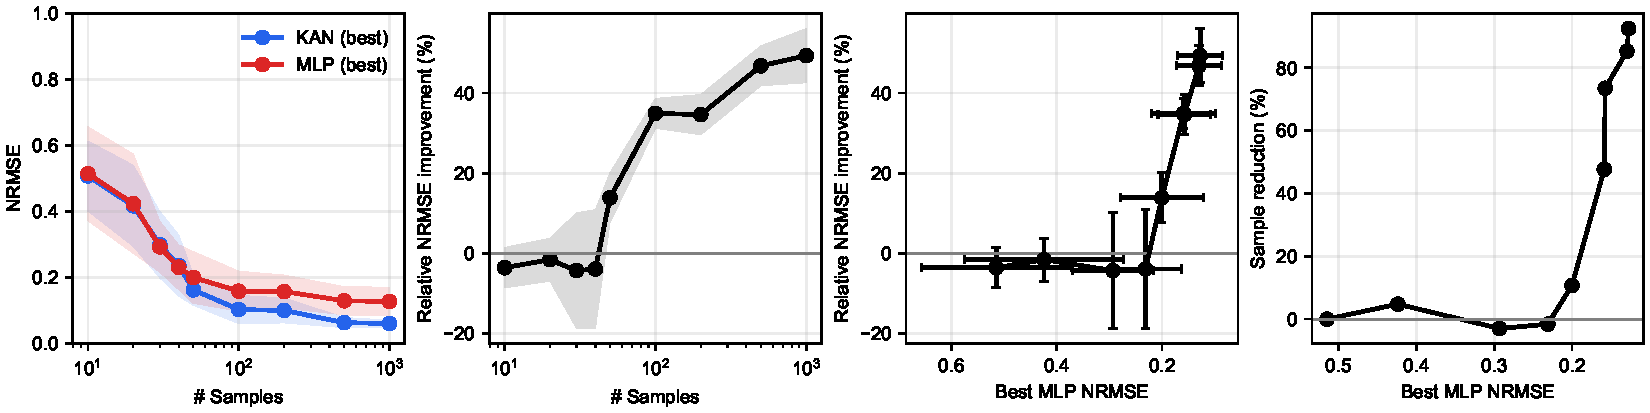
\includegraphics[width=\linewidth]{figures/Figure_X1_2.pdf}
    \caption{Experiment 1: Sample Efficiency in Feynman Benchmark.}
    \label{fig:result_exp1}
\end{figure}

\begin{figure}[!h]
    \centering
    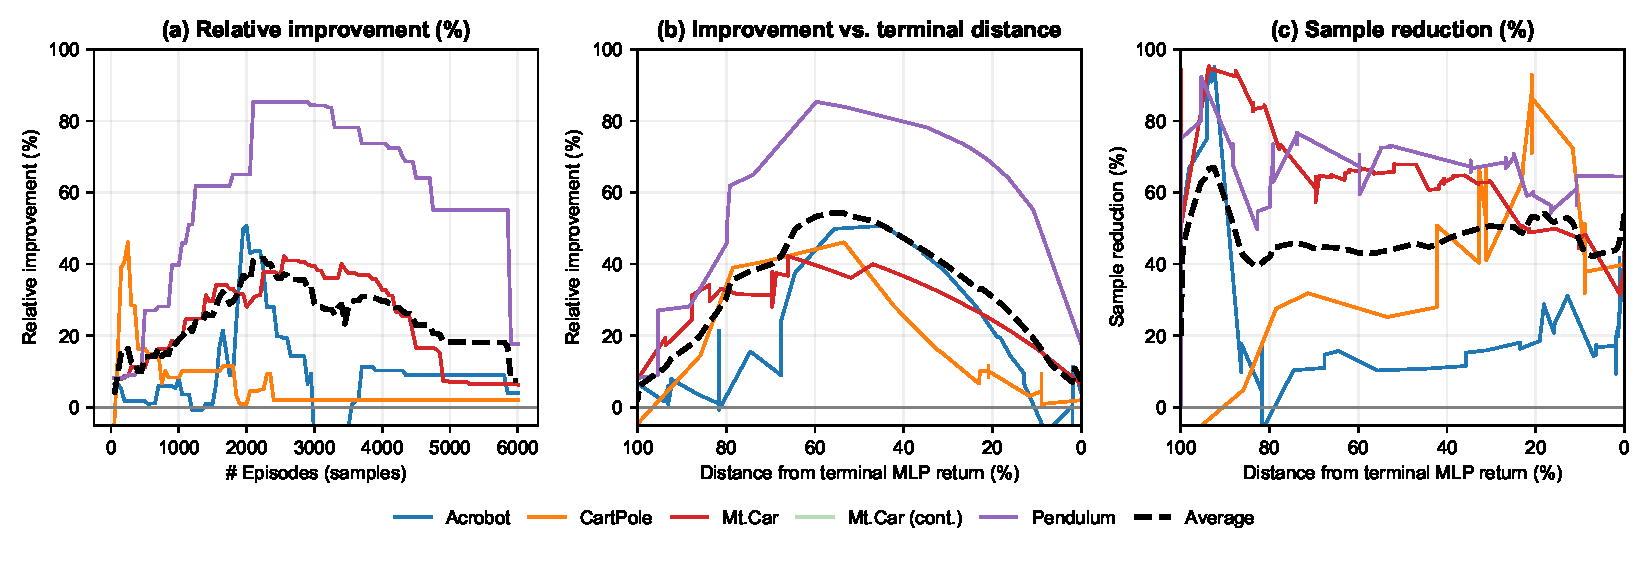
\includegraphics[width=\linewidth]{figures/Figure_X2_2.pdf}
    \caption{Experiment 2: Sample Efficiency in Gymnasium Benchmark.}
    \label{fig:result_exp2}
\end{figure}



%%%%%%%%%%%%%%%%%%%%%%%%%%%%%%%%%%%%%%%%%%%%%%%%%%%%%%%%%%%%
\section{Discussion}

% Results are encouraging further experiments with more complex control and robotics problems.
% Results are also encouraging hybrid learning strategies, where computationally-less efficient KANs are used to learn as much as possible from few observed samples, and later on distilled to MLP for faster inference.
Overall, the experiments support the claim that KAN architectures can improve sample efficiency when the task contains smooth low-dimensional structures.
The strongest gains occur in the early and middle part of training, which is the regime that matters most when simulator calls, measurements, or hardware trials are expensive.
The effect is not uniform across tasks, and the final returns are often close once both model architectures receive many samples.
The results suggest that KANs can be useful for low-data control problems.
A practical route for deployment is to train with KANs during the scarce-sample phase and then distill the learned policy into a cheaper MLP when inference cost is the bottleneck.
%The present study is limited to the Feynman benchmark and low-dimensional Gymnasium Classic Control tasks, so larger continuous-control, robotic, and safety-critical benchmarks remain necessary.
%Future work should separate actor-only and critic-only effects, test stricter parameter matching, and measure wall-clock cost alongside environment-sample efficiency.


%%%%%%%%%%%%%%%%%%%%%%%%%%%%%%%%%%%%%%%%%%%%%%%%%%%%%%%%%%%%
\newpage
% \section*{References}

% References follow the acknowledgments in the camera-ready paper. Use unnumbered first-level heading for
% the references. Any choice of citation style is acceptable as long as you are
% consistent. It is permissible to reduce the font size to \verb+small+ (9 point)
% when listing the references.
% Note that the Reference section does not count towards the page limit.
% \medskip

\bibliographystyle{unsrt}
\bibliography{references}




%%%%%%%%%%%%%%%%%%%%%%%%%%%%%%%%%%%%%%%%%%%%%%%%%%%%%%%%%%%%
\clearpage
\appendix

\section{Experiment Setup Details}

\subsection{Feynman Benchmark Details}

\subsubsection{Dataset Construction}

The Feynman benchmark consists of analytic equations with named input variables and prescribed sampling ranges \cite{udrescu2020aifeynman,udrescu2020aifeynman2}.
Following Liu et al., we use the `Feynman\_no\_units' subset and keep all equations for which finite train and test samples can be generated \cite{liu2024kan}
This includes univariate equations, which are reported separately from multivariate equations in the aggregate analysis.
We use the unit-free subset, because univariate equations provide a sanity check for spline-based edge learning, while multivariate equations test whether KANs retain any sample-efficiency advantage when the model must learn interactions between variables.
For each equation $f_j:\mathbb{R}^{d_j}\rightarrow\mathbb{R}$, we generate supervised examples by sampling $x\sim\mathcal{U}(\mathcal{D}_j)$ and evaluating $y=f_j(x)$.
The domain $\mathcal{D}_j$ is the Cartesian product of the variable intervals specified by the benchmark.
Training and test sets are sampled independently for every random seed.
If an equation is undefined at a sampled point or returns a non-finite value, we reject the point and resample until the desired split size is reached.
This rejection step is applied before normalization and is identical for all models.

\subsubsection{Sample-Efficiency Protocol}

For each equation, we fix $N_{\mathrm{test}}=1000$.
We vary the training size over
\[
N_{\mathrm{train}}\in\{10,20,50,100,200,500,1000\}.
\]
For each $N_{\mathrm{train}}$, equation, and model family, we repeat the experiment over $S$ random seeds.
Each seed determines the training draw, the test draw, and the model initialization.
Inputs are standardized using the mean and standard deviation of the training set.
Targets may be standardized during optimization, but all reported metrics are computed after transforming predictions back to the original target scale.
No information from the test set is used for model selection or normalization.

\subsubsection{Model Comparisons}

The main comparison includes KAN and MLP regressors trained with the same optimizer, loss, maximum number of update steps, batch size, and random seeds.
For KANs, we use spline-based edge functions as in the original KAN implementation, with spline order and grid size fixed across equations unless otherwise stated.
For MLPs, we use smooth activations such as SiLU to avoid giving KANs an artificial advantage over nonsmooth ReLU baselines on smooth physics equations.
We report trainable parameter counts and wall-clock training time for every trained model.
The primary setting uses a fixed architecture recipe for each model family.
A secondary parameter-matched setting chooses MLP widths so that the number of trainable parameters is as close as possible to the KAN parameter count.
When exact matching is impossible, we report the parameter ratio alongside the result.
This protocol avoids treating parameter count as interchangeable across architectures while still checking whether apparent sample-efficiency gains are explained by model size.

\subsubsection{KAN Implementations}

To validate KAN baselines, we use the public All-KAN implementation repository as the implementation source for several KAN variants.
The implementation collection is organized around the original KAN model and the KAN 2.0 scientific-discovery framework \cite{liu2024kan,liu2024kan2}.
Our experiment wrapper currently exposes EfficientKAN for B-spline KANs, FastKAN for Gaussian RBF edge functions, and BSRBF-KAN for hybrid B-spline/RBF edge functions \cite{li2024kolmogorovarnold,ta2024bsrbf}.
The All-KAN repository also includes recent variants such as FC-KAN, PRKAN, and AF-KAN, which provide implementation references for future ablations \cite{ta2024fc,ta2025prkan,ta2025afkan}.
All implementation choices are fixed across sample budgets within an experiment, and each reported result specifies the backend used to instantiate the KAN model.

\subsubsection{Metrics}

Let $\{(x_i,y_i)\}_{i=1}^{N_{\mathrm{test}}}$ be the test set for one equation and let $\hat{y}_i$ be the model prediction.
We define the test-set mean and standard deviation as
\[
\bar{y}=\frac{1}{N_{\mathrm{test}}}\sum_{i=1}^{N_{\mathrm{test}}}y_i,
\qquad
s_y=\sqrt{\frac{1}{N_{\mathrm{test}}}\sum_{i=1}^{N_{\mathrm{test}}}(y_i-\bar{y})^2}.
\]
The root mean squared error is
\[
\mathrm{RMSE}=\sqrt{\frac{1}{N_{\mathrm{test}}}\sum_{i=1}^{N_{\mathrm{test}}}(\hat{y}_i-y_i)^2}.
\]
The normalized root mean squared error is
\[
\mathrm{NRMSE}=\frac{\mathrm{RMSE}}{s_y+\epsilon},
\]
where $\epsilon=10^{-12}$ prevents numerical instability for nearly constant targets.
The mean absolute error is
\[
\mathrm{MAE}=\frac{1}{N_{\mathrm{test}}}\sum_{i=1}^{N_{\mathrm{test}}}|\hat{y}_i-y_i|.
\]
The relative $\ell_2$ error is
\[
\mathrm{Rel}\text{-}\ell_2=\frac{\sqrt{\sum_{i=1}^{N_{\mathrm{test}}}(\hat{y}_i-y_i)^2}}{\sqrt{\sum_{i=1}^{N_{\mathrm{test}}}y_i^2}+\epsilon}.
\]
The coefficient of determination is
\[
R^2=1-\frac{\sum_{i=1}^{N_{\mathrm{test}}}(\hat{y}_i-y_i)^2}{\sum_{i=1}^{N_{\mathrm{test}}}(y_i-\bar{y})^2+\epsilon}.
\]
RMSE and MAE preserve the physical scale of each equation.
NRMSE and relative $\ell_2$ error allow comparisons across equations with different output magnitudes.
$R^2$ reports explained variance and is easier to interpret when communicating whether a model has learned the dominant structure of the function.

\subsubsection{Aggregate Reporting}

For each equation and training size, we report the mean and standard error over seeds.
Across equations, we report the median and interquartile range rather than only the mean, since a small number of high-scale or ill-conditioned equations can dominate aggregate errors.
We report these aggregate statistics for all equations, for univariate equations only, and for multivariate equations only.
The full sample-efficiency curve plots NRMSE against $N_{\mathrm{train}}$ on a logarithmic x-axis.
As scalar summaries, we report the area under the error-sample curve and the sample threshold $N_\tau$.
The area under the error-sample curve is computed by trapezoidal integration of NRMSE over $\log N_{\mathrm{train}}$, where lower values indicate better sample efficiency.
The threshold $N_\tau$ is the smallest training-set size for which the median NRMSE falls below a chosen target $\tau$.
If no method reaches $\tau$, we report $N_\tau>1000$.

\subsection{RL Gymnasium Benchmark Details}

\subsubsection{Benchmark and Agents}

We use the Gymnasium Classic Control environments CartPole-v1, Acrobot-v1, MountainCar-v0, MountainCarContinuous-v0, and Pendulum-v1.
The observations are low-dimensional state vectors, which matches the intended use of KAN edge functions for smooth physical relationships.
The runner supports both discrete and continuous action spaces, using categorical policies for discrete actions and diagonal Gaussian policies with tanh squashing for continuous actions.
For continuous actions, the trainable log standard deviation is initialized to $0$.

\subsubsection{Model Sweep}

The main comparison uses full actor-critic agents, so the actor and critic are both KANs for KAN runs and both MLPs for MLP runs.
The KAN sweep includes B-spline KANs and Gaussian RBF KANs with hidden dimensions $[2]$, $[4]$, $[8]$, $[4,4]$, $[8,8]$, and $[16,16]$.
The MLP sweep includes ReLU and sigmoid MLPs with hidden dimensions $[16]$, $[32]$, $[64]$, $[32,32]$, and $[64,64]$.
The KAN settings use grid size $5$, spline order $3$, grid range $[-1.5,1.5]$, and SiLU as the base activation.
The runner records actor, critic, and total trainable parameter counts for every checkpoint.
% TALK ABOUT IMPLEMENTATION, HOW IS MLP implemented, how KAN; what python package used?
% Justify model sweep in one sentence: we tested models of different complexity, finding that higher complexities do not yield benefits

\subsubsection{PPO Training and Evaluation}

Each training job collects complete episodes, computes generalized advantage estimates with $\gamma=0.99$ and $\lambda=0.95$, and applies clipped PPO updates with clip parameter $0.20$.
The optimizer is Adam with learning rate $3\times10^{-4}$, no weight decay, entropy coefficient $0.01$, value coefficient $0.50$, four PPO epochs per update, and gradient clipping at $0.50$.
Updates are performed after batches of five episodes in the full protocol.
Training seeds are paired across model families, and evaluation uses deterministic actions with five evaluation episodes per checkpoint.
Discrete policies are evaluated with the action of maximum logit, while continuous policies are evaluated with the mean action.
The result file used for the paper contains ten paired random seeds and learning curves up to 6000 training episodes.
During training, episodes, cumulative environment steps, recent training returns, deterministic evaluation returns, episode lengths, PPO losses, runtime, and parameter counts are logged.
% Justify training in one sentence: say we tried to optimize the hyperparameter of training process via grid search, to enable both MLP and KAN the best possible performance during learning

\subsection{RL Gymnasium Noise Benchmark Details}

\subsubsection{Reward Perturbation}

The noisy benchmark keeps the same Gymnasium environments, PPO update, model sweep, and deterministic clean evaluation protocol as the clean Gymnasium benchmark.
During training only, each clean reward $r_t$ is replaced by $r_t^{\mathrm{noise}}=r_t+\alpha\epsilon_t$, where $\epsilon_t\sim\mathcal{N}(0,1)$.
The main sweep uses $\alpha\in\{0,0.25,0.5,1,2,4,7,10\}$ in raw reward units.
Because noise only enters the rewards used for advantage estimation, the experiment tests robustness to corrupted training feedback rather than robustness to stochastic evaluation.

\clearpage
\section{Detailed Results}

\begin{figure}[!h]
    \centering
    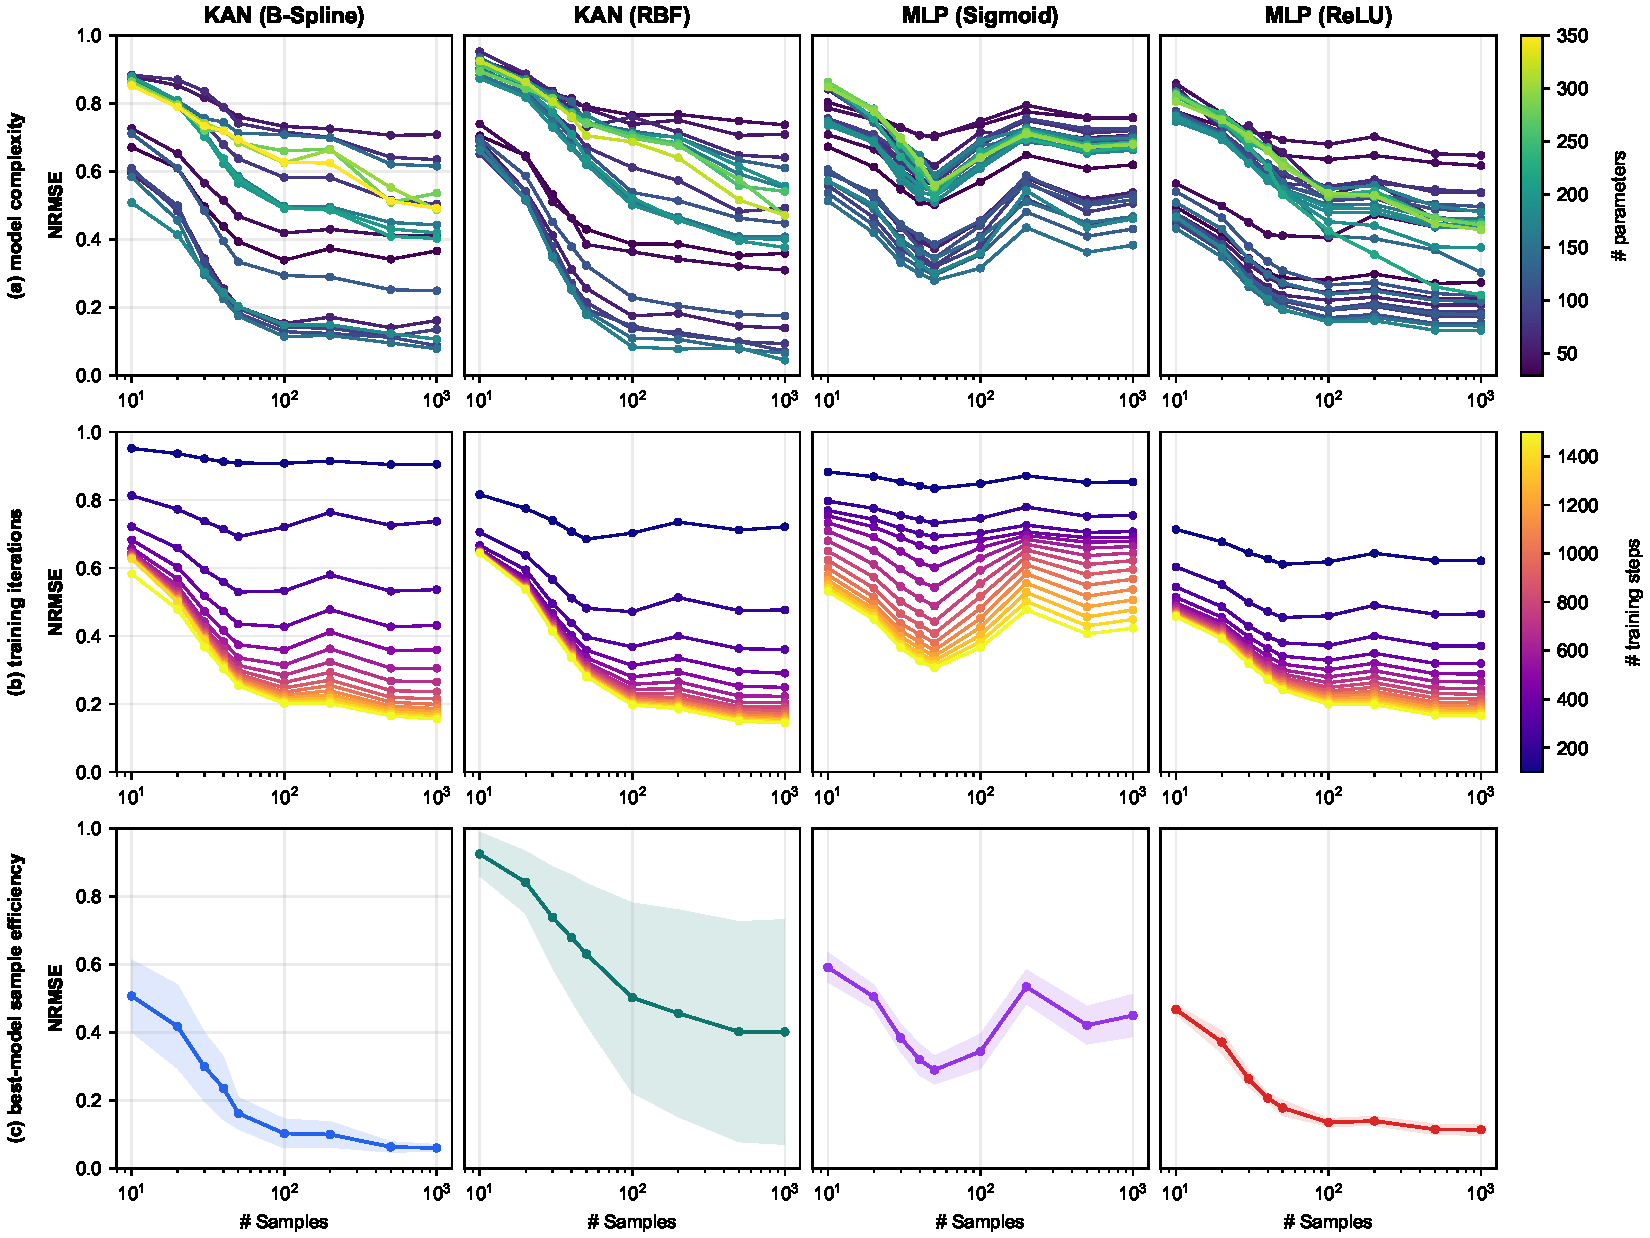
\includegraphics[width=\linewidth]{figures/Figure_X1_1.pdf}
    \caption{Experiment 1: Feynman Benchmark Experiment Design.}
    \label{fig:experiment_1_results}
\end{figure}

\begin{figure}[!h]
    \centering
    \rotatebox{270}{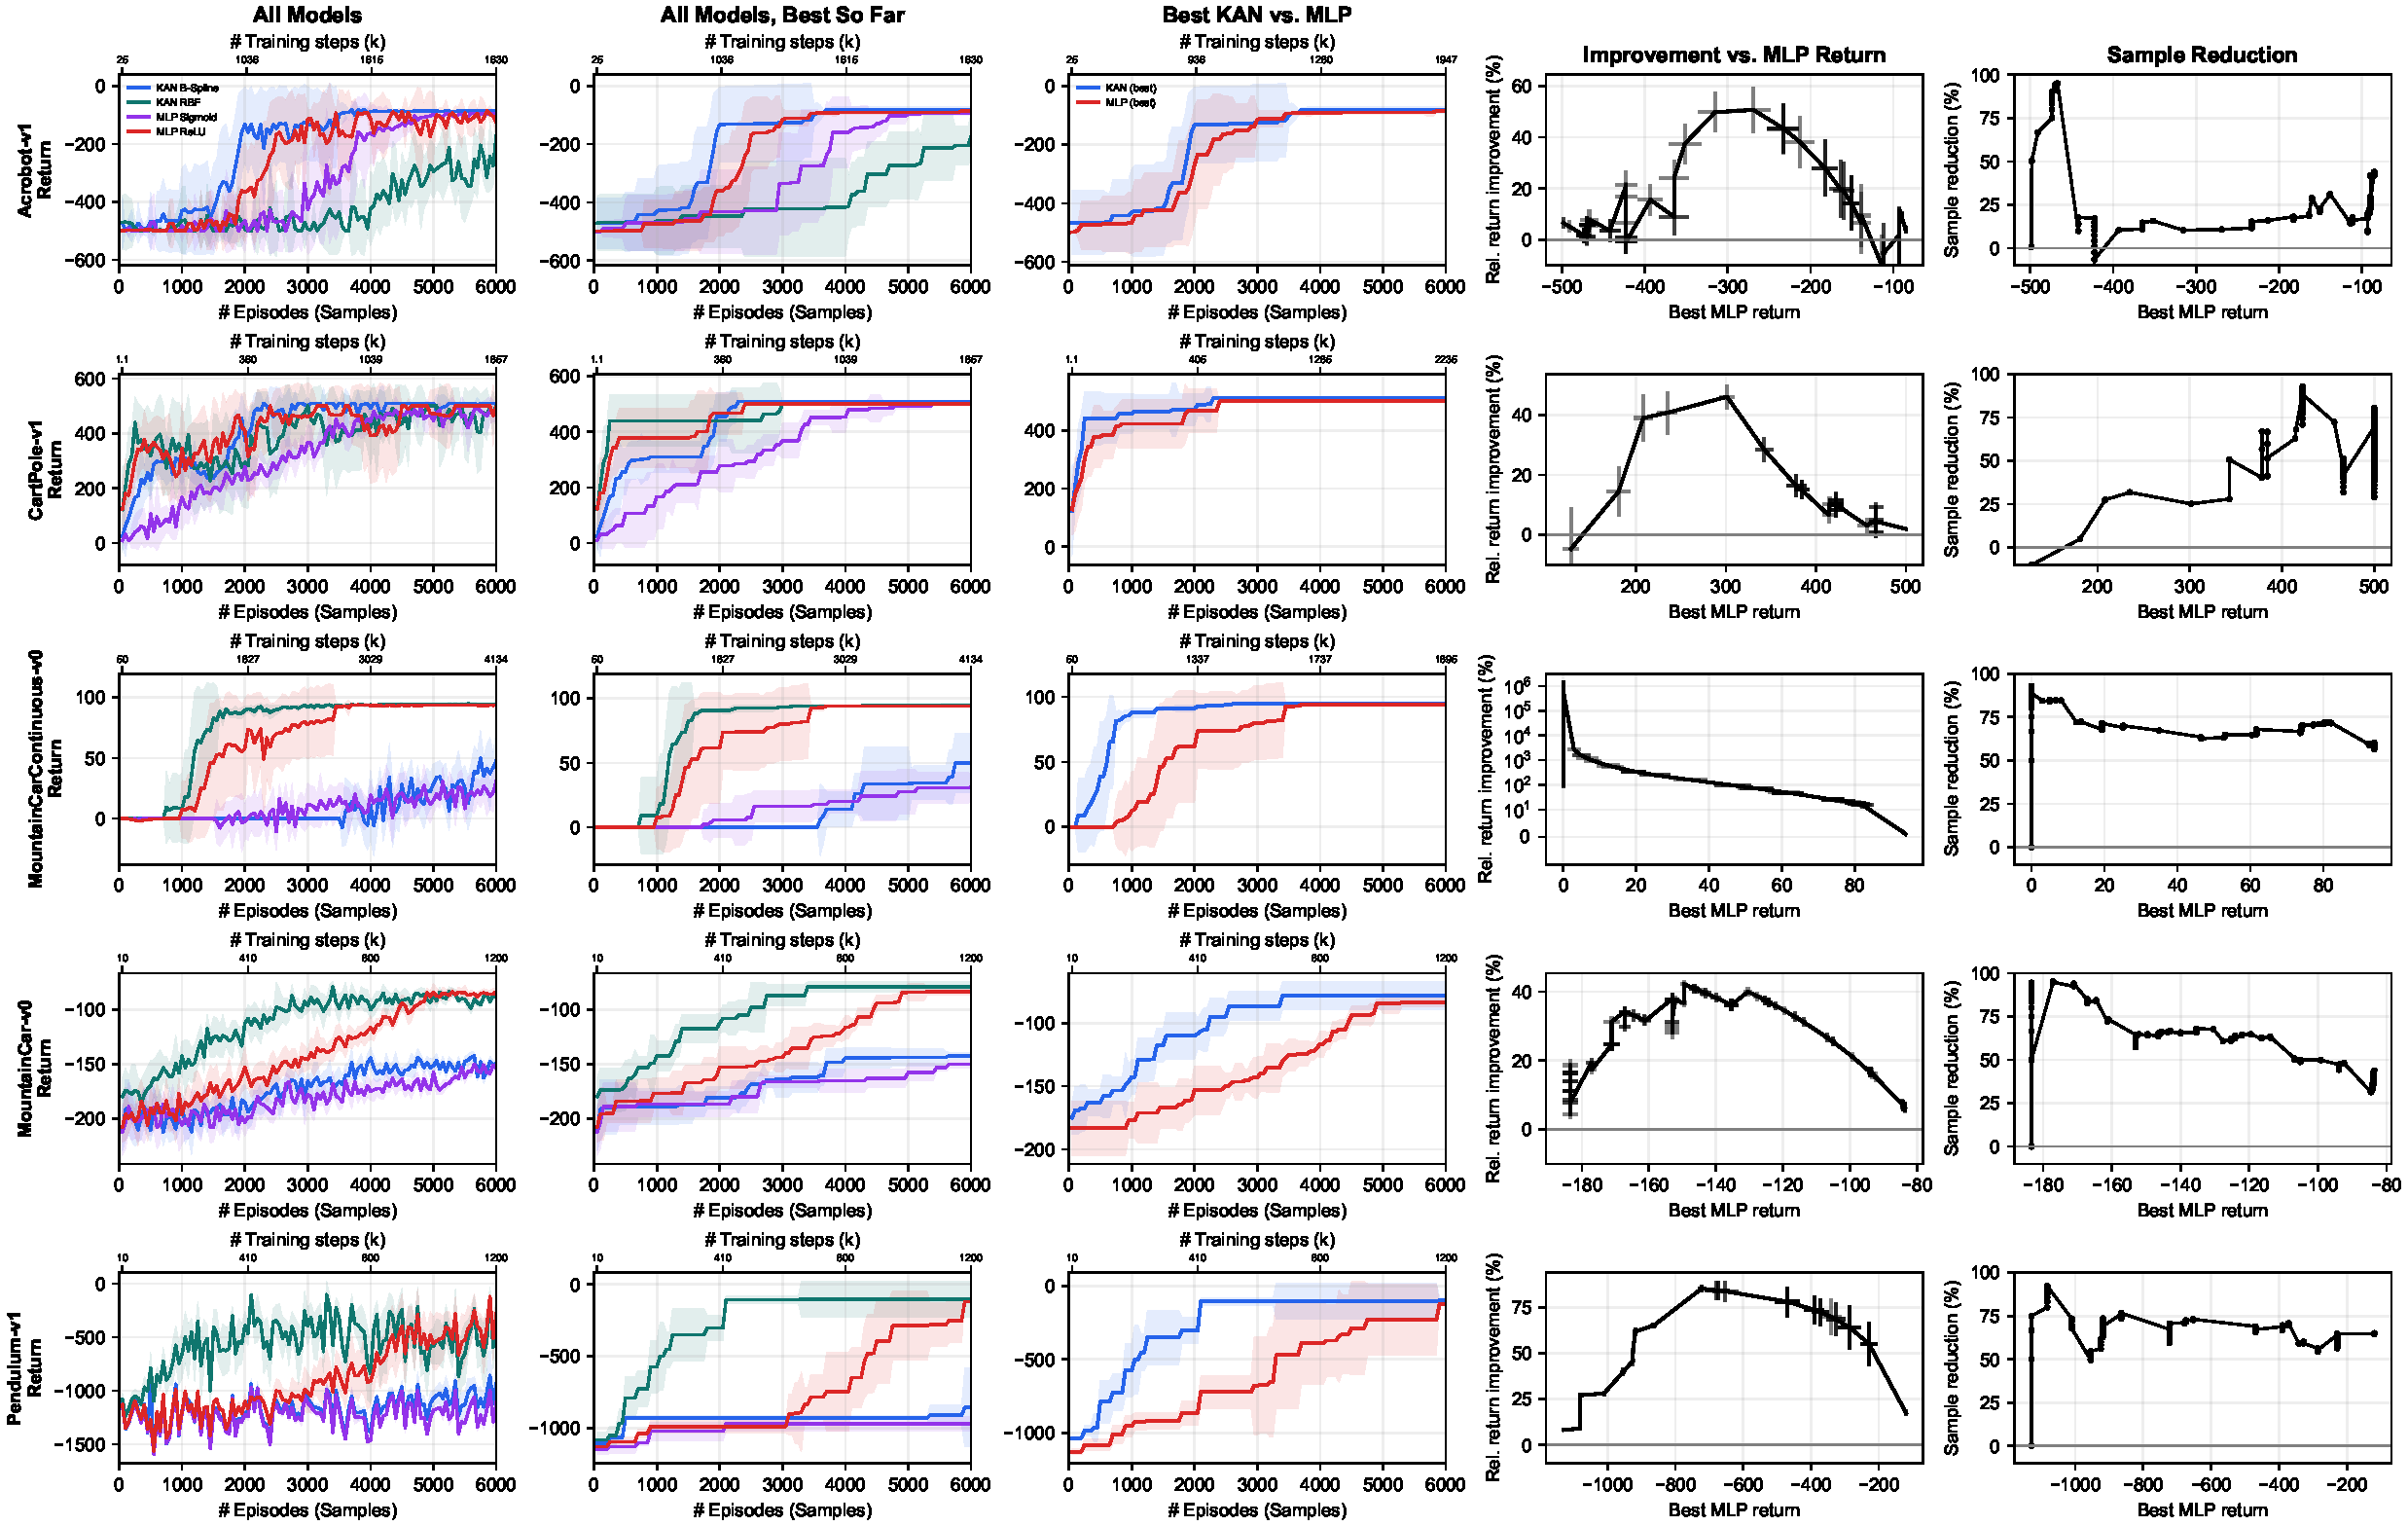
\includegraphics[width=1.5\linewidth]{figures/Figure_X2_1.pdf}}
    \caption{Experiment 2: DeepRL Gymnasium Experiment Design.}
    \label{fig:experiment_2_results}
\end{figure}

\begin{figure}[!h]
    \centering
    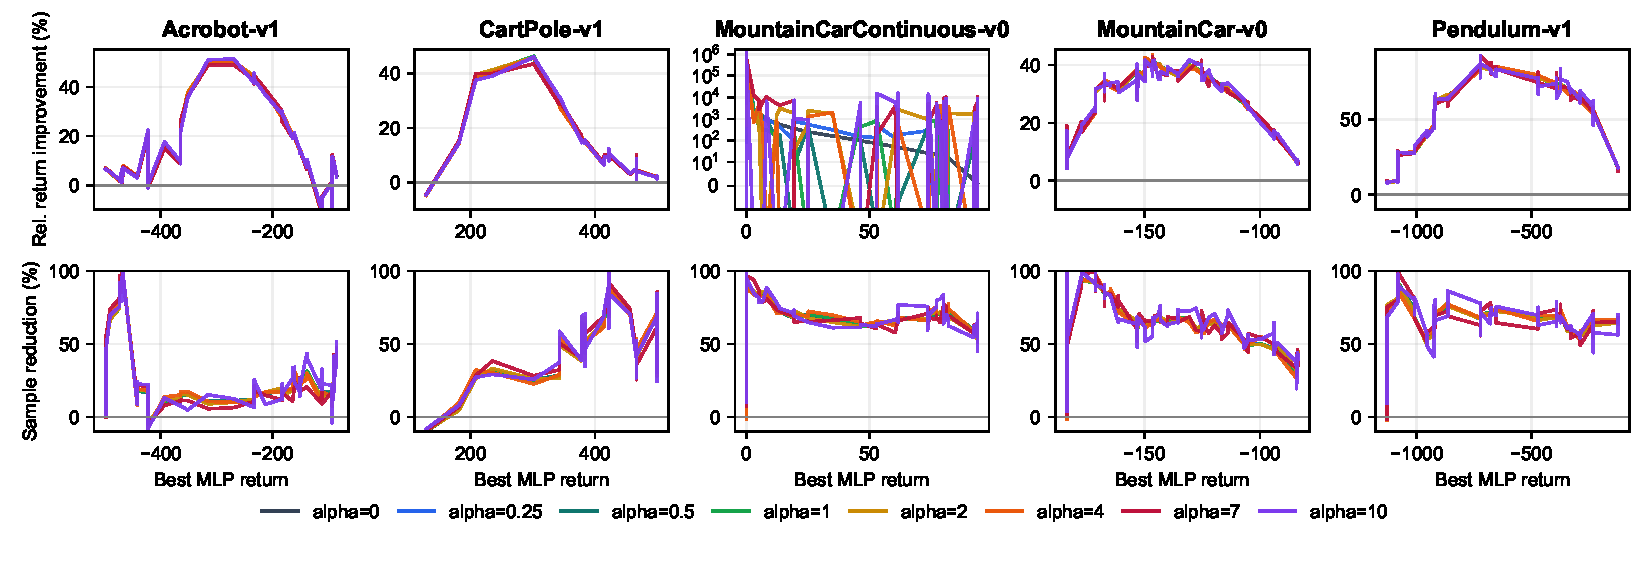
\includegraphics[width=\linewidth]{figures/Figure_X3_3.pdf}
    \caption{Experiment 3: Sample Efficiency in Noised Gymnasium Benchmark.}
    \label{fig:result_exp3}
\end{figure}

%%%%%%%%%%%%%%%%%%%%%%%%%%%%%%%%%%%%%%%%%%%%%%%%%%%%%%%%%%%%

% \newpage
% \section*{NeurIPS Paper Checklist}

%%% BEGIN INSTRUCTIONS %%%
The checklist is designed to encourage best practices for responsible machine learning research, addressing issues of reproducibility, transparency, research ethics, and societal impact. Do not remove the checklist: {\bf The papers not including the checklist will be desk rejected.} The checklist should follow the references and follow the (optional) supplemental material.  The checklist does NOT count towards the page
limit. 

Please read the checklist guidelines carefully for information on how to answer these questions. For each question in the checklist:
\begin{itemize}
    \item You should answer \answerYes{}, \answerNo{}, or \answerNA{}.
    \item \answerNA{} means either that the question is Not Applicable for that particular paper or the relevant information is Not Available.
    \item Please provide a short (1--2 sentence) justification right after your answer (even for \answerNA). 
   % \item {\bf The papers not including the checklist will be desk rejected.}
\end{itemize}

{\bf The checklist answers are an integral part of your paper submission.} They are visible to the reviewers, area chairs, senior area chairs, and ethics reviewers. You will also be asked to include it (after eventual revisions) with the final version of your paper, and its final version will be published with the paper.

The reviewers of your paper will be asked to use the checklist as one of the factors in their evaluation. While \answerYes{} is generally preferable to \answerNo{}, it is perfectly acceptable to answer \answerNo{} provided a proper justification is given (e.g., error bars are not reported because it would be too computationally expensive'' or ``we were unable to find the license for the dataset we used''). In general, answering \answerNo{} or \answerNA{} is not grounds for rejection. While the questions are phrased in a binary way, we acknowledge that the true answer is often more nuanced, so please just use your best judgment and write a justification to elaborate. All supporting evidence can appear either in the main paper or the supplemental material, provided in appendix. If you answer \answerYes{} to a question, in the justification please point to the section(s) where related material for the question can be found.

IMPORTANT, please:
\begin{itemize}
    \item {\bf Delete this instruction block, but keep the section heading ``NeurIPS Paper Checklist"},
    \item  {\bf Keep the checklist subsection headings, questions/answers and guidelines below.}
    \item {\bf Do not modify the questions and only use the provided macros for your answers}.
\end{itemize} 
 

%%% END INSTRUCTIONS %%%


\begin{enumerate}

\item {\bf Claims}
    \item[] Question: Do the main claims made in the abstract and introduction accurately reflect the paper's contributions and scope?
    \item[] Answer: \answerTODO{} % Replace by \answerYes{}, \answerNo{}, or \answerNA{}.
    \item[] Justification: \justificationTODO{}
    \item[] Guidelines:
    \begin{itemize}
        \item The answer \answerNA{} means that the abstract and introduction do not include the claims made in the paper.
        \item The abstract and/or introduction should clearly state the claims made, including the contributions made in the paper and important assumptions and limitations. A \answerNo{} or \answerNA{} answer to this question will not be perceived well by the reviewers. 
        \item The claims made should match theoretical and experimental results, and reflect how much the results can be expected to generalize to other settings. 
        \item It is fine to include aspirational goals as motivation as long as it is clear that these goals are not attained by the paper. 
    \end{itemize}

\item {\bf Limitations}
    \item[] Question: Does the paper discuss the limitations of the work performed by the authors?
    \item[] Answer: \answerTODO{} % Replace by \answerYes{}, \answerNo{}, or \answerNA{}.
    \item[] Justification: \justificationTODO{}
    \item[] Guidelines:
    \begin{itemize}
        \item The answer \answerNA{} means that the paper has no limitation while the answer \answerNo{} means that the paper has limitations, but those are not discussed in the paper. 
        \item The authors are encouraged to create a separate ``Limitations'' section in their paper.
        \item The paper should point out any strong assumptions and how robust the results are to violations of these assumptions (e.g., independence assumptions, noiseless settings, model well-specification, asymptotic approximations only holding locally). The authors should reflect on how these assumptions might be violated in practice and what the implications would be.
        \item The authors should reflect on the scope of the claims made, e.g., if the approach was only tested on a few datasets or with a few runs. In general, empirical results often depend on implicit assumptions, which should be articulated.
        \item The authors should reflect on the factors that influence the performance of the approach. For example, a facial recognition algorithm may perform poorly when image resolution is low or images are taken in low lighting. Or a speech-to-text system might not be used reliably to provide closed captions for online lectures because it fails to handle technical jargon.
        \item The authors should discuss the computational efficiency of the proposed algorithms and how they scale with dataset size.
        \item If applicable, the authors should discuss possible limitations of their approach to address problems of privacy and fairness.
        \item While the authors might fear that complete honesty about limitations might be used by reviewers as grounds for rejection, a worse outcome might be that reviewers discover limitations that aren't acknowledged in the paper. The authors should use their best judgment and recognize that individual actions in favor of transparency play an important role in developing norms that preserve the integrity of the community. Reviewers will be specifically instructed to not penalize honesty concerning limitations.
    \end{itemize}

\item {\bf Theory assumptions and proofs}
    \item[] Question: For each theoretical result, does the paper provide the full set of assumptions and a complete (and correct) proof?
    \item[] Answer: \answerTODO{} % Replace by \answerYes{}, \answerNo{}, or \answerNA{}.
    \item[] Justification: \justificationTODO{}
    \item[] Guidelines:
    \begin{itemize}
        \item The answer \answerNA{} means that the paper does not include theoretical results. 
        \item All the theorems, formulas, and proofs in the paper should be numbered and cross-referenced.
        \item All assumptions should be clearly stated or referenced in the statement of any theorems.
        \item The proofs can either appear in the main paper or the supplemental material, but if they appear in the supplemental material, the authors are encouraged to provide a short proof sketch to provide intuition. 
        \item Inversely, any informal proof provided in the core of the paper should be complemented by formal proofs provided in appendix or supplemental material.
        \item Theorems and Lemmas that the proof relies upon should be properly referenced. 
    \end{itemize}

    \item {\bf Experimental result reproducibility}
    \item[] Question: Does the paper fully disclose all the information needed to reproduce the main experimental results of the paper to the extent that it affects the main claims and/or conclusions of the paper (regardless of whether the code and data are provided or not)?
    \item[] Answer: \answerTODO{} % Replace by \answerYes{}, \answerNo{}, or \answerNA{}.
    \item[] Justification: \justificationTODO{}
    \item[] Guidelines:
    \begin{itemize}
        \item The answer \answerNA{} means that the paper does not include experiments.
        \item If the paper includes experiments, a \answerNo{} answer to this question will not be perceived well by the reviewers: Making the paper reproducible is important, regardless of whether the code and data are provided or not.
        \item If the contribution is a dataset and\slash or model, the authors should describe the steps taken to make their results reproducible or verifiable. 
        \item Depending on the contribution, reproducibility can be accomplished in various ways. For example, if the contribution is a novel architecture, describing the architecture fully might suffice, or if the contribution is a specific model and empirical evaluation, it may be necessary to either make it possible for others to replicate the model with the same dataset, or provide access to the model. In general. releasing code and data is often one good way to accomplish this, but reproducibility can also be provided via detailed instructions for how to replicate the results, access to a hosted model (e.g., in the case of a large language model), releasing of a model checkpoint, or other means that are appropriate to the research performed.
        \item While NeurIPS does not require releasing code, the conference does require all submissions to provide some reasonable avenue for reproducibility, which may depend on the nature of the contribution. For example
        \begin{enumerate}
            \item If the contribution is primarily a new algorithm, the paper should make it clear how to reproduce that algorithm.
            \item If the contribution is primarily a new model architecture, the paper should describe the architecture clearly and fully.
            \item If the contribution is a new model (e.g., a large language model), then there should either be a way to access this model for reproducing the results or a way to reproduce the model (e.g., with an open-source dataset or instructions for how to construct the dataset).
            \item We recognize that reproducibility may be tricky in some cases, in which case authors are welcome to describe the particular way they provide for reproducibility. In the case of closed-source models, it may be that access to the model is limited in some way (e.g., to registered users), but it should be possible for other researchers to have some path to reproducing or verifying the results.
        \end{enumerate}
    \end{itemize}


\item {\bf Open access to data and code}
    \item[] Question: Does the paper provide open access to the data and code, with sufficient instructions to faithfully reproduce the main experimental results, as described in supplemental material?
    \item[] Answer: \answerTODO{} % Replace by \answerYes{}, \answerNo{}, or \answerNA{}.
    \item[] Justification: \justificationTODO{}
    \item[] Guidelines:
    \begin{itemize}
        \item The answer \answerNA{} means that paper does not include experiments requiring code.
        \item Please see the NeurIPS code and data submission guidelines (\url{https://neurips.cc/public/guides/CodeSubmissionPolicy}) for more details.
        \item While we encourage the release of code and data, we understand that this might not be possible, so \answerNo{} is an acceptable answer. Papers cannot be rejected simply for not including code, unless this is central to the contribution (e.g., for a new open-source benchmark).
        \item The instructions should contain the exact command and environment needed to run to reproduce the results. See the NeurIPS code and data submission guidelines (\url{https://neurips.cc/public/guides/CodeSubmissionPolicy}) for more details.
        \item The authors should provide instructions on data access and preparation, including how to access the raw data, preprocessed data, intermediate data, and generated data, etc.
        \item The authors should provide scripts to reproduce all experimental results for the new proposed method and baselines. If only a subset of experiments are reproducible, they should state which ones are omitted from the script and why.
        \item At submission time, to preserve anonymity, the authors should release anonymized versions (if applicable).
        \item Providing as much information as possible in supplemental material (appended to the paper) is recommended, but including URLs to data and code is permitted.
    \end{itemize}


\item {\bf Experimental setting/details}
    \item[] Question: Does the paper specify all the training and test details (e.g., data splits, hyperparameters, how they were chosen, type of optimizer) necessary to understand the results?
    \item[] Answer: \answerTODO{} % Replace by \answerYes{}, \answerNo{}, or \answerNA{}.
    \item[] Justification: \justificationTODO{}
    \item[] Guidelines:
    \begin{itemize}
        \item The answer \answerNA{} means that the paper does not include experiments.
        \item The experimental setting should be presented in the core of the paper to a level of detail that is necessary to appreciate the results and make sense of them.
        \item The full details can be provided either with the code, in appendix, or as supplemental material.
    \end{itemize}

\item {\bf Experiment statistical significance}
    \item[] Question: Does the paper report error bars suitably and correctly defined or other appropriate information about the statistical significance of the experiments?
    \item[] Answer: \answerTODO{} % Replace by \answerYes{}, \answerNo{}, or \answerNA{}.
    \item[] Justification: \justificationTODO{}
    \item[] Guidelines:
    \begin{itemize}
        \item The answer \answerNA{} means that the paper does not include experiments.
        \item The authors should answer \answerYes{} if the results are accompanied by error bars, confidence intervals, or statistical significance tests, at least for the experiments that support the main claims of the paper.
        \item The factors of variability that the error bars are capturing should be clearly stated (for example, train/test split, initialization, random drawing of some parameter, or overall run with given experimental conditions).
        \item The method for calculating the error bars should be explained (closed form formula, call to a library function, bootstrap, etc.)
        \item The assumptions made should be given (e.g., Normally distributed errors).
        \item It should be clear whether the error bar is the standard deviation or the standard error of the mean.
        \item It is OK to report 1-sigma error bars, but one should state it. The authors should preferably report a 2-sigma error bar than state that they have a 96\% CI, if the hypothesis of Normality of errors is not verified.
        \item For asymmetric distributions, the authors should be careful not to show in tables or figures symmetric error bars that would yield results that are out of range (e.g., negative error rates).
        \item If error bars are reported in tables or plots, the authors should explain in the text how they were calculated and reference the corresponding figures or tables in the text.
    \end{itemize}

\item {\bf Experiments compute resources}
    \item[] Question: For each experiment, does the paper provide sufficient information on the computer resources (type of compute workers, memory, time of execution) needed to reproduce the experiments?
    \item[] Answer: \answerTODO{} % Replace by \answerYes{}, \answerNo{}, or \answerNA{}.
    \item[] Justification: \justificationTODO{}
    \item[] Guidelines:
    \begin{itemize}
        \item The answer \answerNA{} means that the paper does not include experiments.
        \item The paper should indicate the type of compute workers CPU or GPU, internal cluster, or cloud provider, including relevant memory and storage.
        \item The paper should provide the amount of compute required for each of the individual experimental runs as well as estimate the total compute. 
        \item The paper should disclose whether the full research project required more compute than the experiments reported in the paper (e.g., preliminary or failed experiments that didn't make it into the paper). 
    \end{itemize}
    
\item {\bf Code of ethics}
    \item[] Question: Does the research conducted in the paper conform, in every respect, with the NeurIPS Code of Ethics \url{https://neurips.cc/public/EthicsGuidelines}?
    \item[] Answer: \answerTODO{} % Replace by \answerYes{}, \answerNo{}, or \answerNA{}.
    \item[] Justification: \justificationTODO{}
    \item[] Guidelines:
    \begin{itemize}
        \item The answer \answerNA{} means that the authors have not reviewed the NeurIPS Code of Ethics.
        \item If the authors answer \answerNo, they should explain the special circumstances that require a deviation from the Code of Ethics.
        \item The authors should make sure to preserve anonymity (e.g., if there is a special consideration due to laws or regulations in their jurisdiction).
    \end{itemize}


\item {\bf Broader impacts}
    \item[] Question: Does the paper discuss both potential positive societal impacts and negative societal impacts of the work performed?
    \item[] Answer: \answerTODO{} % Replace by \answerYes{}, \answerNo{}, or \answerNA{}.
    \item[] Justification: \justificationTODO{}
    \item[] Guidelines:
    \begin{itemize}
        \item The answer \answerNA{} means that there is no societal impact of the work performed.
        \item If the authors answer \answerNA{} or \answerNo, they should explain why their work has no societal impact or why the paper does not address societal impact.
        \item Examples of negative societal impacts include potential malicious or unintended uses (e.g., disinformation, generating fake profiles, surveillance), fairness considerations (e.g., deployment of technologies that could make decisions that unfairly impact specific groups), privacy considerations, and security considerations.
        \item The conference expects that many papers will be foundational research and not tied to particular applications, let alone deployments. However, if there is a direct path to any negative applications, the authors should point it out. For example, it is legitimate to point out that an improvement in the quality of generative models could be used to generate Deepfakes for disinformation. On the other hand, it is not needed to point out that a generic algorithm for optimizing neural networks could enable people to train models that generate Deepfakes faster.
        \item The authors should consider possible harms that could arise when the technology is being used as intended and functioning correctly, harms that could arise when the technology is being used as intended but gives incorrect results, and harms following from (intentional or unintentional) misuse of the technology.
        \item If there are negative societal impacts, the authors could also discuss possible mitigation strategies (e.g., gated release of models, providing defenses in addition to attacks, mechanisms for monitoring misuse, mechanisms to monitor how a system learns from feedback over time, improving the efficiency and accessibility of ML).
    \end{itemize}
    
\item {\bf Safeguards}
    \item[] Question: Does the paper describe safeguards that have been put in place for responsible release of data or models that have a high risk for misuse (e.g., pre-trained language models, image generators, or scraped datasets)?
    \item[] Answer: \answerTODO{} % Replace by \answerYes{}, \answerNo{}, or \answerNA{}.
    \item[] Justification: \justificationTODO{}
    \item[] Guidelines:
    \begin{itemize}
        \item The answer \answerNA{} means that the paper poses no such risks.
        \item Released models that have a high risk for misuse or dual-use should be released with necessary safeguards to allow for controlled use of the model, for example by requiring that users adhere to usage guidelines or restrictions to access the model or implementing safety filters. 
        \item Datasets that have been scraped from the Internet could pose safety risks. The authors should describe how they avoided releasing unsafe images.
        \item We recognize that providing effective safeguards is challenging, and many papers do not require this, but we encourage authors to take this into account and make a best faith effort.
    \end{itemize}

\item {\bf Licenses for existing assets}
    \item[] Question: Are the creators or original owners of assets (e.g., code, data, models), used in the paper, properly credited and are the license and terms of use explicitly mentioned and properly respected?
    \item[] Answer: \answerTODO{} % Replace by \answerYes{}, \answerNo{}, or \answerNA{}.
    \item[] Justification: \justificationTODO{}
    \item[] Guidelines:
    \begin{itemize}
        \item The answer \answerNA{} means that the paper does not use existing assets.
        \item The authors should cite the original paper that produced the code package or dataset.
        \item The authors should state which version of the asset is used and, if possible, include a URL.
        \item The name of the license (e.g., CC-BY 4.0) should be included for each asset.
        \item For scraped data from a particular source (e.g., website), the copyright and terms of service of that source should be provided.
        \item If assets are released, the license, copyright information, and terms of use in the package should be provided. For popular datasets, \url{paperswithcode.com/datasets} has curated licenses for some datasets. Their licensing guide can help determine the license of a dataset.
        \item For existing datasets that are re-packaged, both the original license and the license of the derived asset (if it has changed) should be provided.
        \item If this information is not available online, the authors are encouraged to reach out to the asset's creators.
    \end{itemize}

\item {\bf New assets}
    \item[] Question: Are new assets introduced in the paper well documented and is the documentation provided alongside the assets?
    \item[] Answer: \answerTODO{} % Replace by \answerYes{}, \answerNo{}, or \answerNA{}.
    \item[] Justification: \justificationTODO{}
    \item[] Guidelines:
    \begin{itemize}
        \item The answer \answerNA{} means that the paper does not release new assets.
        \item Researchers should communicate the details of the dataset\slash code\slash model as part of their submissions via structured templates. This includes details about training, license, limitations, etc. 
        \item The paper should discuss whether and how consent was obtained from people whose asset is used.
        \item At submission time, remember to anonymize your assets (if applicable). You can either create an anonymized URL or include an anonymized zip file.
    \end{itemize}

\item {\bf Crowdsourcing and research with human subjects}
    \item[] Question: For crowdsourcing experiments and research with human subjects, does the paper include the full text of instructions given to participants and screenshots, if applicable, as well as details about compensation (if any)? 
    \item[] Answer: \answerTODO{} % Replace by \answerYes{}, \answerNo{}, or \answerNA{}.
    \item[] Justification: \justificationTODO{}
    \item[] Guidelines:
    \begin{itemize}
        \item The answer \answerNA{} means that the paper does not involve crowdsourcing nor research with human subjects.
        \item Including this information in the supplemental material is fine, but if the main contribution of the paper involves human subjects, then as much detail as possible should be included in the main paper. 
        \item According to the NeurIPS Code of Ethics, workers involved in data collection, curation, or other labor should be paid at least the minimum wage in the country of the data collector. 
    \end{itemize}

\item {\bf Institutional review board (IRB) approvals or equivalent for research with human subjects}
    \item[] Question: Does the paper describe potential risks incurred by study participants, whether such risks were disclosed to the subjects, and whether Institutional Review Board (IRB) approvals (or an equivalent approval/review based on the requirements of your country or institution) were obtained?
    \item[] Answer: \answerTODO{} % Replace by \answerYes{}, \answerNo{}, or \answerNA{}.
    \item[] Justification: \justificationTODO{}
    \item[] Guidelines:
    \begin{itemize}
        \item The answer \answerNA{} means that the paper does not involve crowdsourcing nor research with human subjects.
        \item Depending on the country in which research is conducted, IRB approval (or equivalent) may be required for any human subjects research. If you obtained IRB approval, you should clearly state this in the paper. 
        \item We recognize that the procedures for this may vary significantly between institutions and locations, and we expect authors to adhere to the NeurIPS Code of Ethics and the guidelines for their institution. 
        \item For initial submissions, do not include any information that would break anonymity (if applicable), such as the institution conducting the review.
    \end{itemize}

\item {\bf Declaration of LLM usage}
    \item[] Question: Does the paper describe the usage of LLMs if it is an important, original, or non-standard component of the core methods in this research? Note that if the LLM is used only for writing, editing, or formatting purposes and does \emph{not} impact the core methodology, scientific rigor, or originality of the research, declaration is not required.
    %this research? 
    \item[] Answer: \answerTODO{} % Replace by \answerYes{}, \answerNo{}, or \answerNA{}.
    \item[] Justification: \justificationTODO{}
    \item[] Guidelines:
    \begin{itemize}
        \item The answer \answerNA{} means that the core method development in this research does not involve LLMs as any important, original, or non-standard components.
        \item Please refer to our LLM policy in the NeurIPS handbook for what should or should not be described.
    \end{itemize}

\end{enumerate}


\end{document}
